%% LyX 2.1.4 created this file.  For more info, see http://www.lyx.org/.
%% Do not edit unless you really know what you are doing.
\documentclass[10pt,english]{article}
\usepackage{ae,aecompl}
\usepackage[T1]{fontenc}
\usepackage[latin9]{inputenc}
\usepackage{geometry}
\usepackage{graphicx}
\graphicspath{{Figures/}}
\usepackage{float}
\geometry{verbose,tmargin=.5in,bmargin=.5in,lmargin=.5in,rmargin=.5in}
\setlength{\parskip}{\smallskipamount}
\setlength{\parindent}{0pt}
\usepackage{amsmath,tabu}
\usepackage{amsthm,url}
\usepackage{amssymb}
\usepackage{hyperref}
\usepackage{comment}
\hypersetup{colorlinks,urlcolor=blue,citecolor=blue,linkcolor=blue}
\usepackage{hhline}
%line spacing
\usepackage{setspace}
\setstretch{1.25}
\addtolength{\topmargin}{.9in}
\addtolength{\textheight}{-1.1in}
\makeatletter
%%%%%%%%%%%%%%%%%%%%%%%%%%%%%% Textclass specific LaTeX commands.
\theoremstyle{plain}
\ifx\thechapter\undefined
\newtheorem{thm}{\protect\theoremname}
\else
\newtheorem{thm}{\protect\theoremname}[chapter]
\fi
  \theoremstyle{remark}
  \newtheorem{rem}
[thm]{\protect\remarkname
}

\makeatother

\usepackage{babel}
  \providecommand{\remarkname}{Remark}
\providecommand{\theoremname}{Theorem}


\begin{document}

\title{ECON 326: The Economics of Developing Countries \\
$ $\\
Midterm Exam}
\date{80 minutes}
\maketitle
Please do not open the exam until you are instructed to do so. Write your name on this page and every additional book that you use. The entire exam is worth 75 points, with point values assigned as a roughly suggested amount of time spent on each question. None of the answers are intended to require more than 3-5 sentences, with many requiring no more than a sentence or two. You do not need to write in complete sentences as long as the idea is clear (e.g. bullet points are sufficient). \textbf{Read each question carefully and be sure to answer each part.}


\newpage

\section{Literature Review (34 points)}
\subsection{Poverty Traps (6 points)}
Fafchamps et al. (2013) randomly provided cash and in-kind grants to male- and female-owned microenterprises in Ghana. In the table below, the dependent variable is real monthly profits, and the relevant independent variables are listed. The omitted group is the control group. For each variable in (i)-(iii), answer whether the effect on profits for men and women pooled was (statistically) positive, negative, or zero, then provide the intuition as to why this was the case.
        \begin{figure}[ht]
            \centering
            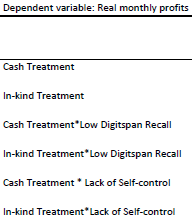
\includegraphics[trim={0 3cm 0 0},clip]{fafchamps_self_control2.png}\\
            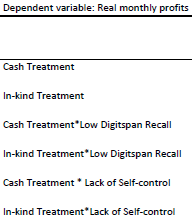
\includegraphics[trim={0 0 0 4.4cm},clip]{fafchamps_self_control2.png}
        \end{figure}

       
        \begin{itemize}
            \item[(i)] (2 pts) In-kind Treatment
            \\
            \textbf{Solution:} The variable has a statistically positive coefficient. For those \textit{with} self-control (i.e., whenever the ``Lack of Self-contorl'' dummy equals zero), the in-kind treatment raises profits. This means that the grants are being used properly for the improvement of these microenterprises, at least in part. 
            \vspace{1cm}
            \item[(ii)] (2 pts) Cash Treatment * Lack of Self-control
            \\
            \textbf{Solution:} The variable has a statistically negative coefficient. This means that, relative to people who receive the cash treatment \textit{and} have self-control, those who receive cash and lack self-control realize lower profits. This is consistent with people without self-control misusing the cash grants, possibly consuming them.
            \vspace{1cm}
            \item[(iii)] (2 pts) In-kind Treatment * Lack of Self-control
            \\
            \textbf{Solution:} The variable has a statistically zero coefficient. This means that, those with and without self-control respond similarly to the in-kind grants.
            \vspace{1cm}
        \end{itemize} \newpage
        
\subsection{Fundamental Causes of Development (7 points)}
Acemoglu, Johnson, and Robinson (2001) on ``Colonial Origins'' aims to measure the effect of institutions on economic growth using an instrumental variable (IV) method to address possible endogeneity.
\begin{itemize}
    \item[(a)] (2 pts) Provide one potential source of endogeneity and the direction of the bias that this would generate. 
    \\
    \textbf{Solution:} Answers will vary. For example: growth could cause better institutions instead of the other way around and this will cause OLS estiamtes of the effect of institutions on growth to have upward bias.
    \vspace{5cm}
    \item[(b)] (2 pts) What IV does AJR (2001) use? What does the relevance assumption mean in this context, and what is the channel/mechanism by which AJR argue that the instrument is relevant? 
    \\
    \textbf{Solution:} The instrument is settler mortality. Relevance here means that settler mortality has a strong effect on institutions. AJR argue that settler mortality determines whether Europeans wanted to settle on a country centuries ago. Europeans were more likely to build good institutions in places they would settle and this induces institutional differences which may persist until today.
    \vspace{5cm}
    \item[(c)] (3 pts) Sachs (2001) argues that geography is the key determinant of economic development. Describe one of the main channels through which Sachs argues geography affects development, and discuss how Acemoglu, Johnson, and Robinson (2002) (about the reversal of fortune) argues against it.
    \\
    \begin{enumerate}
        \item[(i)] Geography affects climate, which affects productivity through health/nutrition/the disease environment and work capacity
        \item[(ii)] Geography affects trade/transport costs
        \item[(iii)] Initial gaps were exacerbated by technology, especially in agriculture
    \end{enumerate}
    \textbf{Solution:} Jeffrey Sachs (2001) argues that geography is a fundamental determinant of economic development, primarily through its impact on disease burden. One key channel he emphasizes is the prevalence of tropical diseases, such as malaria, which are more common in regions with hot and humid climates. High disease burdens reduce labor productivity, discourage foreign investment, and limit economic growth by increasing mortality rates and reducing the ability of populations to engage in productive activities. This creates a ''geographic poverty trap,'' where countries in tropical regions struggle to achieve sustained economic development.
    Acemoglu, Johnson, and Robinson (2002) challenge this geographic determinism through their ``Reversal of Fortune'' hypothesis. They argue that historical institutions, rather than geography, are the primary drivers of economic development. They show that many regions that were relatively wealthy in 1500 (such as India and the Aztec and Inca Empires) became poor by the 20th century, while previously underdeveloped regions (such as North America and Australia) became wealthy. This reversal suggests that geography alone cannot explain development outcomes. Instead, they argue that European colonization played a crucial role: in regions with high disease burdens and dense populations, Europeans established extractive institutions that persist today, leading to weak property rights and poor economic performance. In contrast, in areas with lower disease burdens, Europeans settled in large numbers and established inclusive institutions that promoted long-term growth.

    Thus, while Sachs sees geography as a direct constraint on development, Acemoglu, Johnson, and Robinson argue that institutional differences, shaped by historical colonization patterns, are the key drivers of economic divergence.
    \vspace{1cm}
\end{itemize}

\subsection{Health (6 points)}
\begin{itemize}
    \item[(a)] (2 pts) Explain one positive and one negative effect of charging higher prices for health products in developing countries. \vspace{4cm}
    \\
    \textbf{Solution:} Positive: Higher prices can increase the perceived value of a product, select for individuals who are more likely to use it, and reduce wasteful consumption, attract R\& D investment, and increase the quality of products.
    Negative: Higher prices can reduce access to essential health products for low-income individuals, leading to worse health outcomes.
    \item[(b)] (4 pts) Ashraf et al. (2010) and Cohen and Dupas (2010) run similar experiments that test the effects of price differences on Clorin (a water purification solution) and insecticide treated bednets, respectively. What do they find regarding your effects listed in (a)? If either effect differs across the two papers, provide one potential explanation as to why. \vspace{5cm}
    \\
    \textbf{Solution:} Ashraf et al. (2010) find that higher prices for Clorin increase the perceived value of the product, leading to higher usage rates. 
    Cohen and Dupas (2010) find that higher prices for bednets reduce access to the product.
    One possible explanation for the different results could be that Cohen and Dupas study a product that people know well and value highly (bed nets).
    \newpage
\end{itemize}

\subsection{Education (7 points)}
Duflo et al. (2011) evaluates classroom tracking, or placing students of similar ability within the same classroom.
\begin{itemize}
    \item[(a)] (1 pt) What is meant by direct vs. indirect peer effects? 
    \\
    \textbf{Solution:} Direct peer effects are the effect of a student's peers on their own outcomes, while indirect peer effects are the effect of a student's peers on their outcomes through the teacher's behavior.
    \item[(b)] (2 pts) What are their findings about the effect of tracking on test scores for above- and below-median students? \vspace{4cm}
    \\
    \textbf{Solution:} Duflo et al. (2011) find that tracking has a positive effect all students, even the students on the lower end of the pre-test score distribution.
    This effect was persistent.
    With tracking, this leads teachers assigned to the
lower-achievement section to teach closer to the median student's level than those
assigned to the upper section, although teacher effort is higher in the upper section. 
    \item[(c)] (4 pts) In the table below, the dependent variable is the title for each column, and both the independent and dependent variables are measured in standard deviations. How does the table provide evidence of both direct and indirect peer effects? Include reasoning for the different magnitudes across the pre-test score distribution in columns (4) - (6) in your explanation.
    \begin{figure}[h!]
        \centering
        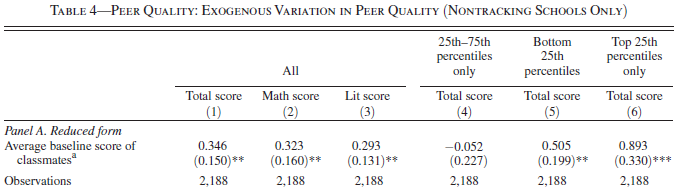
\includegraphics[width=0.75\linewidth]{Figures/duflo_et_al_peer_effects.png}
    \end{figure}

    \textbf{Solution:} 
    The model also has implications for the effects of the test score distribution in
nontracking schools. Specifically, it suggests that an upward shift of the distribution
of peer achievement will strongly raise test scores for a student with initial achievement at the top of the distribution, have an ambiguous impact on scores for a student
closer to the middle, and raise scores at the bottom. This is so because, while all
students benefit from the direct effect of an increase in peer quality, the change in
peer composition also generates an upward shift in the teacher's instruction level.
The higher instruction level will benefit students at the top; hurt those students in the
middle who find themselves further away from the instruction level; and leave the
bottom students unaffected, since they are in any case too far from the target instruction level to benefit from instruction. Estimates exploiting the random assignment
of students to sections in nontracking schools are consistent with these implications
of the model.

    Namely, a uniform increase in peer achievement
increases test scores at the top of the distribution in all cases, but effects on students
in the middle and at the bottom of the distribution depend on whether there are also
direct, positive effects of high-achieving peers. 
In the presence of such effects, the
impact on students in the middle of the distribution is ambiguous, while for those at
the bottom it is positive, albeit weaker than the effects at the top of the distribution.
In the absence of such direct effects, there is a negative impact on students in the
middle of the distribution and no impact at the bottom.
\end{itemize} \newpage


\subsection{Health and Education Relationship (7 points)}
Miguel and Kremer (2004) produce a ``non-experimental'' decomposition of the total treatment effect of de-worming on treated schools into the direct effect on treated students and the spillover on untreated students. What does it mean to be ``non-experimental?'' Summarize the strategy used to identify the effects. \textit{This may be longer than 3-5 sentences, but not too much longer!}

A ``non-experimental'' decomposition means that Miguel and Kremer (2004) did not rely solely on a randomized controlled trial (RCT) to separately estimate the direct and spillover effects of deworming treatment. Instead, they used statistical methods to analyze variations in treatment exposure that were not explicitly randomized at the individual level. While the initial treatment assignment was randomized at the school level, the decomposition of effects relied on observational differences among treated and untreated students within and across schools.

Identification Strategy:
Randomized School Assignment: Schools were randomly assigned to receive deworming treatment in different phases, creating a natural control group.
Direct Effects: The impact on treated students was measured by comparing health and educational outcomes (such as school attendance) between students in treated schools and those in yet-to-be-treated schools.
Spillover Effects (Within-School): Untreated students within treated schools were compared to untreated students in non-treated schools to estimate indirect benefits from reduced transmission.
Spillover Effects (Across-School): Since parasitic infections spread across geographical areas, the study also examined nearby untreated schools to measure cross-school spillovers. Schools close to treated schools were expected to experience lower infection rates, improving outcomes even without direct treatment.
Econometric Adjustments: Since within-school and across-school spillovers were not explicitly randomized, the researchers controlled for potential confounders, such as baseline infection rates and geographic clustering, to better isolate the causal effects.
This non-experimental decomposition allowed Miguel and Kremer to show that deworming had large social benefits, as indirect spillover effects significantly contributed to the overall impact of the program.

The results are non-experimental because treatment was only randomly varied \textit{across} schools.  
Whether someone gets treated or not \textit{within} treated schools is endogenous. 
To disentangle direct and indirect effects, the two mentioned columns split the treated group (Group 1) into treated and untreated students, but doing so may lead to selection biases.  

\newpage

\section{Kremer et al. (2009) and Methods (23 points)}
The Kremer et al. (2009) paper analyzes the effects of offering a merit scholarship program to the top 15\% of Kenyan girls in two districts based on exam scores. They first randomize into control and treatment groups within each district, then compare exam scores between control and treatment. Use the plot below to answer parts (a) and (b).
    \begin{figure}[ht!]
        \centering
        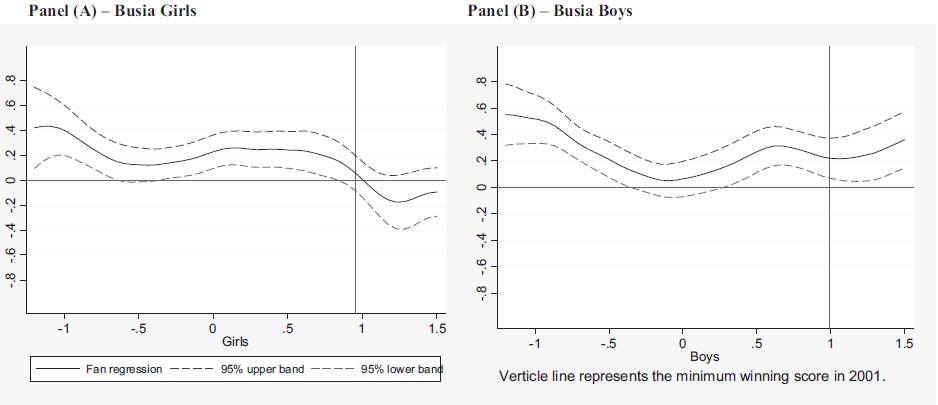
\includegraphics[width=\linewidth]{kremer_busia_effects.png}
    \end{figure}
\begin{itemize}
    \item[(a)] (3 pts) The vertical line represents the cutoff for the top 15\%. In a few sentences, explain what is interesting or perhaps unexpected about the plots, and provide one potential explanation for this pattern based on the education literature.  \vspace{4cm}
    \textbf{Solution:} The scholarship is only for the top performing girls (those to the right of the vertical line in Panel A), but they are the ones who benefit \textit{the least} from the intervention. The education literature shows that people often underestimate the returns to education, so this result could be caused by  the scholarship leading everyone, and not just top performing girls, to update upwards their beliefs about the returns to education. Such belief updates can then lead everyone to put more effort into studying, and maybe top-performing girls are the ones whose scores improve the least in response to this because they were already doing well to begin with.
    \item[(b)] (3 pts) Use your answer from above to answer this question. One of the districts had significant attrition for girls, mostly coming from the upper part of the pretest distribution. Assuming that district had similar effects to the figure, are OLS estimates of the overall treatment effect for girls an overestimate or underestimate of the true effect? Explain. \newpage
    \textbf{Solution:} OLS estimates would be over-estimates of overall (i.e. average) treatment effects because we are removing from the sample those who benefit the least from the intervention. 
\end{itemize} 

Suppose the government of Kenya conducts a similar experiment as in Kremer et al. (2009), except that students scoring at or above an 80 on a writing exam are offered admission to an accelerated-learning (AL) classroom. We are interested in the effect of AL classrooms on post-graduation incomes. We have data on individual exam score ($S_i$), individual AL enrollment ($D_i$ = 1 if enrolled), and logged individual income ($Y_i$), and we consider individuals within 5 points of the cutoff to be ``similar.''


\begin{itemize}
    \item[(c)] (1pt) Write an expression for $T_i$, a dummy for whether the individual is offered AL admission, in terms of the data available. \vspace{2cm}
    \textbf{Solution:} $T_i = 1 $ if and only if $S_i \geq 80$
\end{itemize}
For parts (d) and (e), assume perfect compliance ($T_i = D_i$).
\begin{itemize}
    \item[(d)] (3 pts) Draw a hypothetical figure that depicts $Y_i$ vs. $S_i$. Indicate the size of the treatment effect on the figure, and label this as $TE$. Is this effect an ATE, ITT, ATT, or LATE? Explain. \vspace{3cm}
    \textbf{Solution: } See the graph below. $TE$ is a LATE because it's the effect of the scholarship for those with $S_i=80$.
    \begin{figure}[htbp]
        \centering
        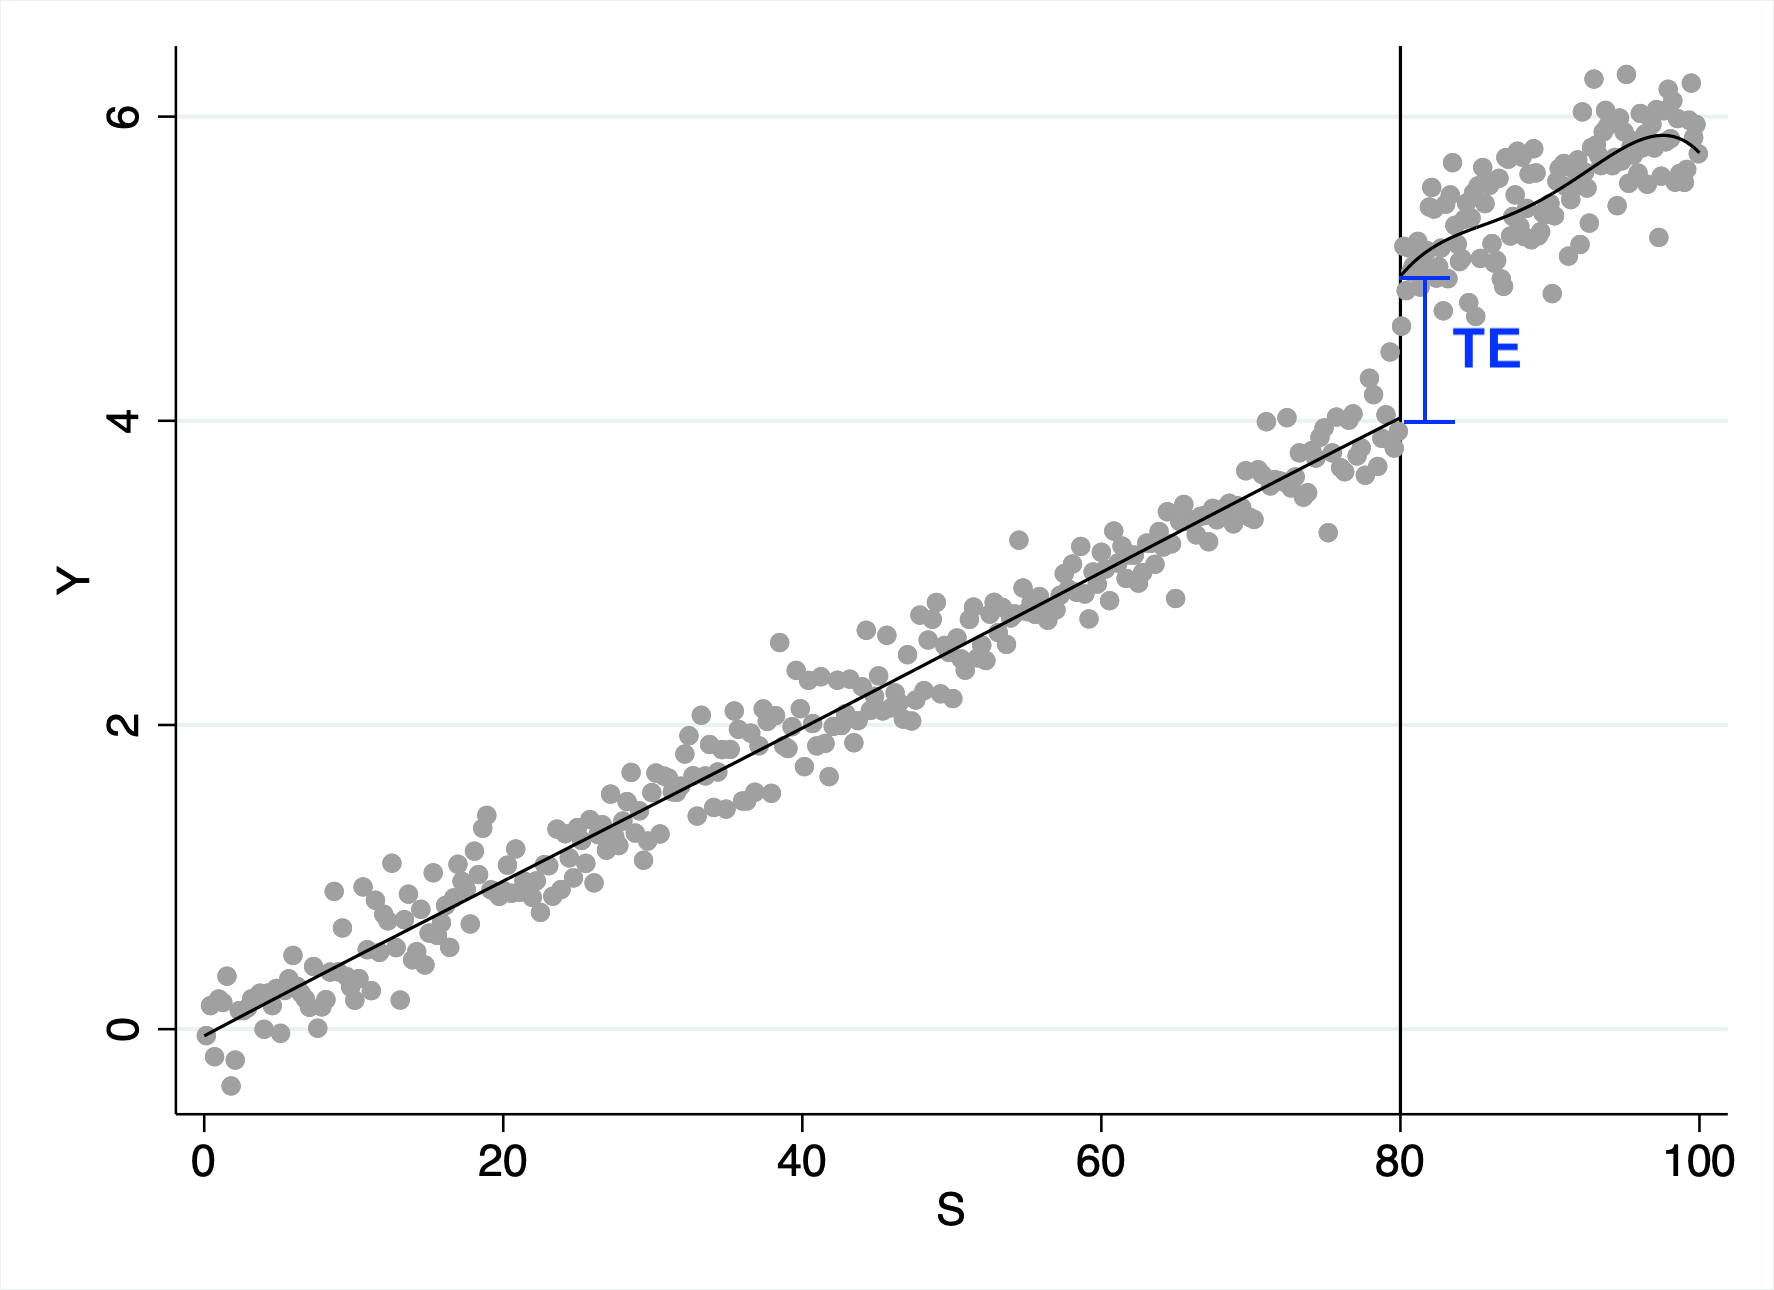
\includegraphics[width=0.6\linewidth]{RDD_PracticeQ2d.png}
    \end{figure}
    \item[(e)] (4 pts) Suppose you learn that after this writing exam, students who finished just below the cutoff received free additional tutoring from the government. Discuss why this would invalidate the RDD strategy. Is $TE$ you estimated from part (d) an over- or underestimate of the true effect of the AL class? Explain in one sentence. \newpage
    
    \textbf{Solution: } The RDD interprets the jump in $Y$ at the $S=80$ cutoff as the treatment effect of the policy. But the additional free tutoring provided to those right below the cutoff would lead the RDD to under-estimate the effects of the scholarship because the positive effects of tutoring artificially attenuate the differences between those right above and below the cutoff. 
\end{itemize}
For the remaining sections, assume there is imperfect compliance ($T_i \neq D_i$): not every student offered admission to the AL classroom takes it up.
\begin{itemize}
    \item[(f)] (5 pts) Suppose the figure you drew in (c) now depicts the relationship between $Y_i$ and $S_i$ with imperfect compliance. Is $TE$ now an ATE, ITT, or ATT? Explain. Is the LATE larger or smaller than $TE$? \vspace{6cm}
    
    \textbf{Solution:} $TE$ now only captures the effect of being offered the scholarship, so it is an ITT. We expect the LATE to be bigger than $TE$ because $LATE=\frac{ITT}{\lambda}$, where the compliance rate $\lambda$ is the effect of being offered the scholarship on the probability of taking it, which is a number between zero and one.
    
    % \item[(g)] (up to 3 bonus pts) Describe how we can econometrically estimate the LATE of the merit scholarship, being specific about the equations used. Describe the population for which this LATE applies to. \textit{This is called a ``Fuzzy RDD'' and we never explicitly covered it in class, but you may be able to reason it out}.
    \item[(g)] (4 pts) Suppose you learn that the distribution of scores is manipulated around the score of 80: students with richer, well-connected parents are graded systematically easier, so that their scores tend to be above 80. Discuss why this would invalidate the RDD strategy. Is $TE$ an over- or underestimate of the true treatment effect of the AL class?
    
    \textbf{Solution:} The RDD strategy relies on the discontinuity in the probability of treatment at the cutoff. If the cutoff is manipulated, the RDD strategy is invalid. $TE$ is an overestimate of the true treatment effect because the manipulation of the cutoff artificially inflates the treatment effect.
\end{itemize}\newpage

\section{Poverty Trap Models and Evidence (18 points)}
For each of the following, draw a graph with $k$ on the x-axis and curves for production, savings, and depreciation and population growth (no need to label them) that produce the corresponding poverty trap using a modified Solow Model framework. On each graph, draw arrows denoting the direction of convergence on the x-axis and label all steady states (e.g. $k_1^*$, $k_2^*$, etc.). Then, provide one reason that justifies the difference between each model and the standard Solow Model. 

The equations for the \textbf{standard} Solow Model are:
\begin{align*}
    y &= Ak^\alpha \ \ &\text{where $0 < \alpha < 1$} \\
    \Delta k &= sy - (\delta+n)k \ \ &\text{where $\Delta$ denotes the change in each period}
\end{align*}
    \begin{itemize}
        \item[(a)] (4 pts) ``Big Push'' poverty trap  \vspace{6.5cm}
        \textbf{Solution:} The figure below displays two stable steady states, $k_1^*$ and $k_3^*$, as well as one unstable steady state $k_2^*$. The model differs from the standard Solow model by introducing non-convexities in the production function, which generate a poverty trap. 
        \begin{figure}[htbp]
        \centering
        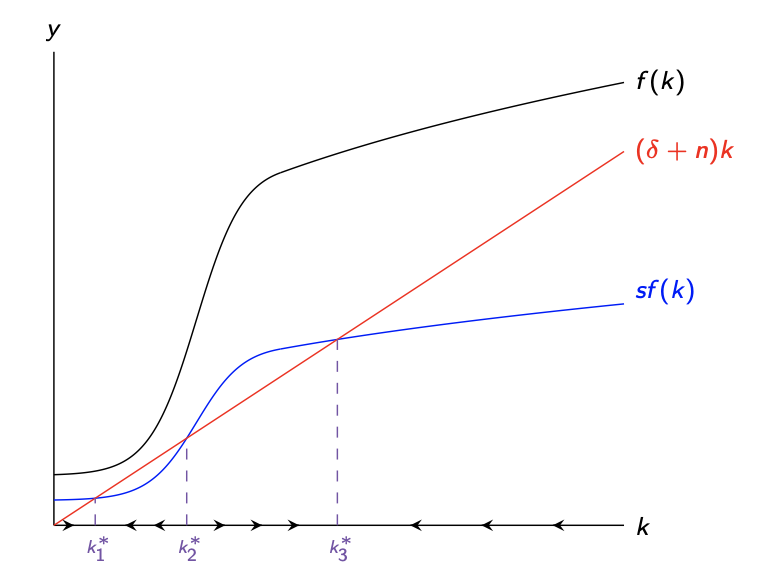
\includegraphics[width=0.25\linewidth]{Q3a.png}
        \end{figure}\\
        \vspace{-1cm}
        \item[(b)] (5 pts) A ``demographic'' poverty trap, in which population growth rate is $n_1$ below capital level $k_{cutoff}$ and $n_2$ above $k_{cutoff}$, where $n_1 > n_2$ (not seen in class). \newpage
        \textbf{Solution:} The figure below also has two stable steady states. The model differs from the standard one by allowing poor countries to exhibit higher fertility rates, which is in line with the data.
        \begin{figure}[htbp]
        \centering
        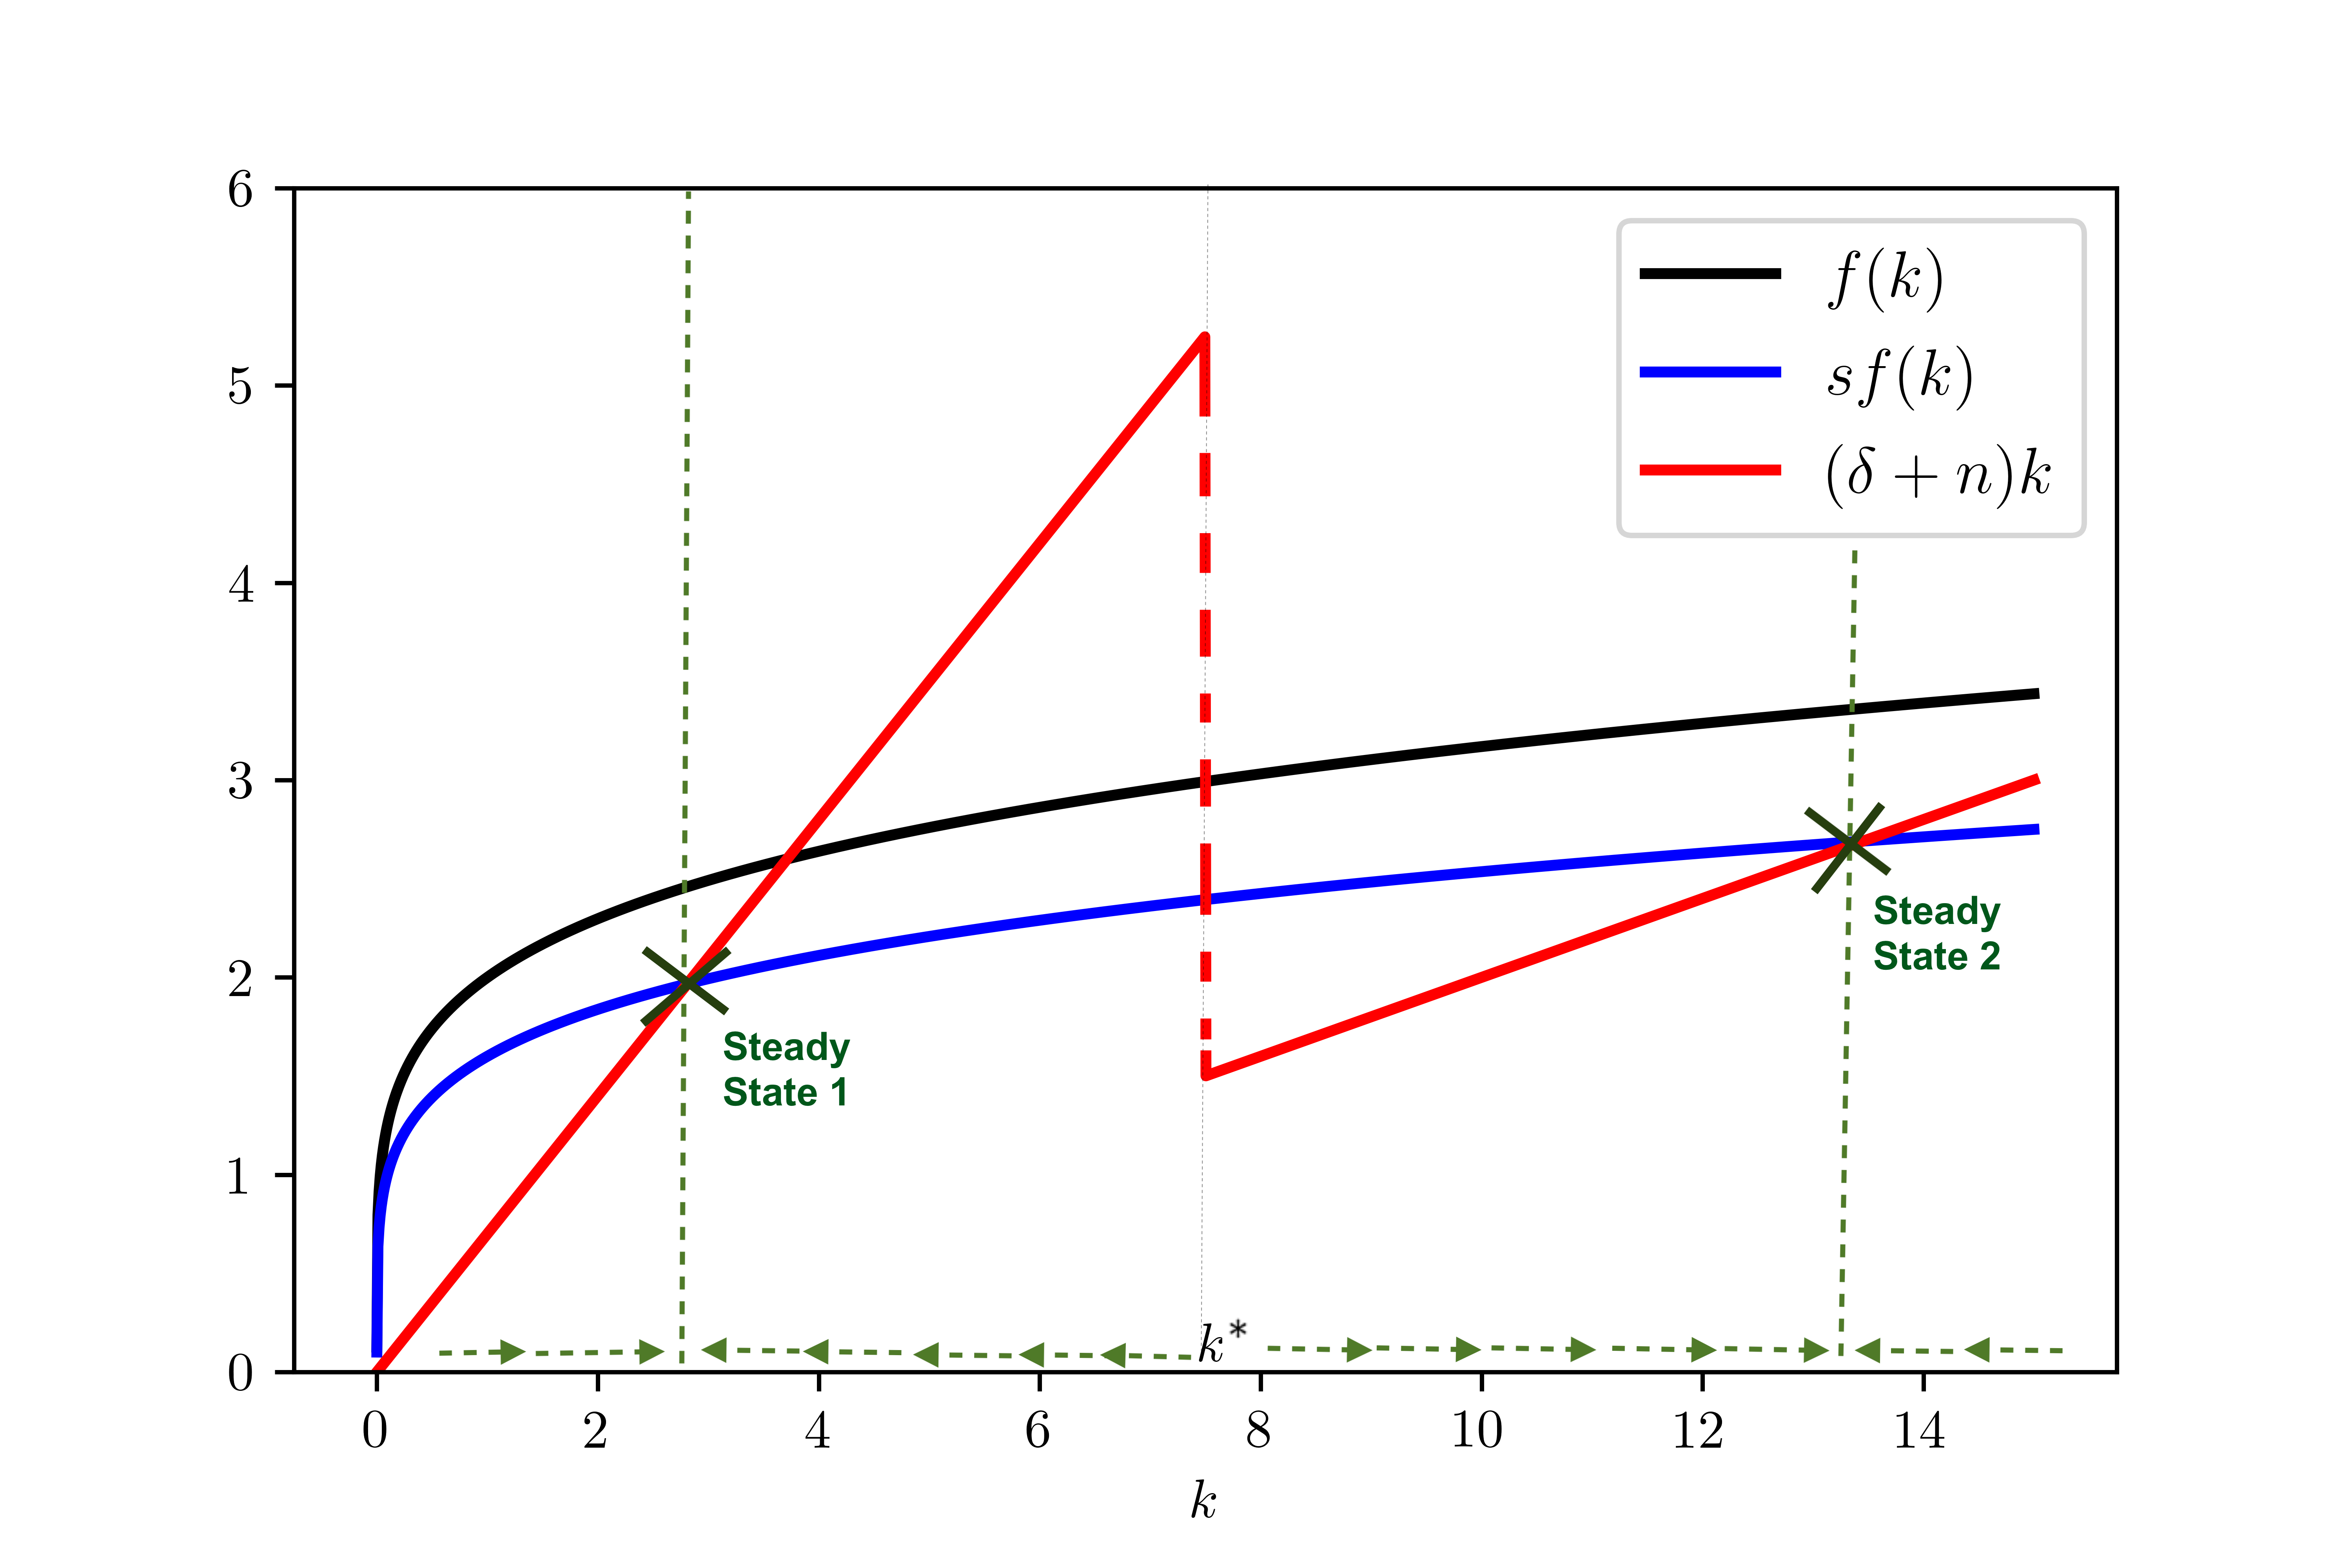
\includegraphics[width=0.3\linewidth]{Q-3-b_edited.png}
        \end{figure}
        \item[(c)] (4 pts) Describe two potential ways that a country can escape the poverty traps drawn above. Choose one of the graphs (be sure to clearly label) and show how each of these ways would change the graph to eliminate the trap(s). \vspace{5cm}
        \textbf{Solution:}  One way is to obtain an external transfer that pushes the country (or every individual in the country) above the required cutoff ($k_2^*$ in question a or $k^*$ in question b). An alternative is to increase productivity. As can be seen in question a's graph, if $f(k)$ experiences an upward shift that is big enough, we can guarantee that the only intersection that remains between the red and blue lines will be $k_3^*$ (modified graph is straightforward and not included here). 
        \item[(d)] (5 pts) Balboni et al. study the existence of individual-level poverty traps. Part of their experiment randomizes 6,000 extremely poor households to receive a \$500 transfer of productive assets. Draw a graph with the treatment group's productive assets in year $t+1$ on the y-axis vs. their productive assets (plus transfer) in year $t$ on the x-axis. Then, add the 45-degree line, and draw a curve that emulates their findings on average productive asset dynamics. Briefly describe how this graph suggests the existence of a poverty trap or a lack thereof.
        \textbf{Solution:} The graph below (taken from the paper) suggests the existence of a poverty trap because the blue curve intersects the 45 degree line three times. Intersections between the blue curve and the 45 degree line indicate that initial and final assets are identical, so three intersections mean that we have three steady states. Moreover, two of these are stable steady states because the blue curve intersects the 45 degree line from above.
        \begin{figure}[htbp]
        \centering
        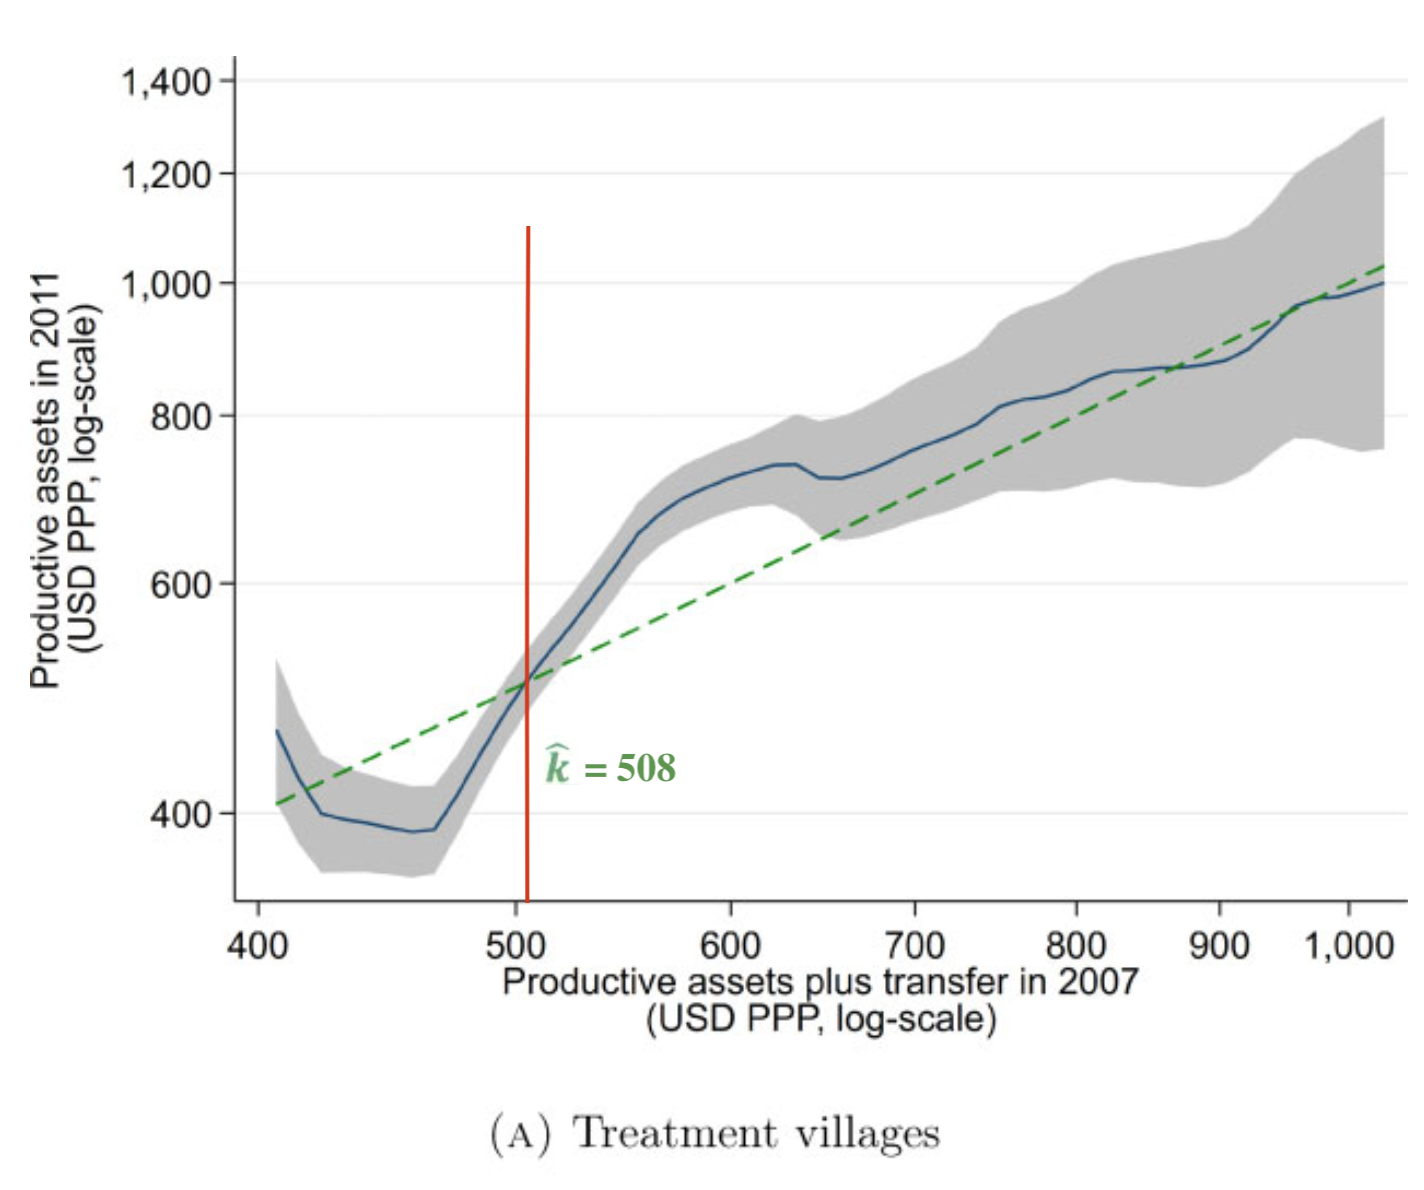
\includegraphics[width=0.8\linewidth]{Q-3-e.png}
        \end{figure}
    \end{itemize} \vspace{7cm}


\end{document}
